\documentclass[a4paper,12pt]{report}
\usepackage[utf-8]{inputenc}
\usepackage{graphicx}
\usepackage{latexsym,a4,epsfig,times}
\usepackage[french]{babel}
\usepackage[T1]{fontenc}
\usepackage{hyperref}
\usepackage{moreverb}
\usepackage{listings}
\usepackage{color}
\usepackage{float}
% \usepackage[top=30mm, bottom=20mm, left=15mm, right=15mm]{geometry}
\usepackage[top=45mm, bottom=45mm, left=15mm, right=15mm]{geometry}
\usepackage{fancyhdr}
\usepackage{pdfpages}
\usepackage{bibtopic}
\usepackage{lscape} 

\definecolor{colKeys}{rgb}{0,0,1}
\definecolor{colIdentifier}{rgb}{0,0,0}
\definecolor{colComments}{rgb}{0,0.5,1}
\definecolor{colString}{rgb}{0.6,0.1,0.1}
\lstset{
basicstyle=\ttfamily\small, %
identifierstyle=\color{colIdentifier}, %
keywordstyle=\color{colKeys}, %
stringstyle=\color{colString}, %
commentstyle=\color{colComments},
language=java,
backgroundcolor=\color{white},
frame=single,                   % adds a frame around the code
tabsize=2,                      % sets default tabsize to 2 spaces
}

\hypersetup{
colorlinks= true,
linkcolor = black,
anchorcolor = black,
citecolor = black,
filecolor = black,
pagecolor = black,
urlcolor = black,
breaklinks=false,
pdfpagemode= UseOutlines,
}
% \setlength{\textheight}{220mm}
\setlength{\textheight}{200mm}
\setlength{\headheight}{14pt}
\fancypagestyle{plain}{
\fancyhf[]{}
}
\title{Refactoring IzPack}
\author{Anthonin Bonnefoy, David Duponchel}
\lstset{language=Java}
\begin{document}
\renewcommand{\chaptername}{Partie}
\renewcommand{\headrulewidth}{0pt}
\makeatother
%---------------------------------------
\begin{titlepage}
~
\vfill
\begin{center}
\textsc{\begin{LARGE}TP - Métadonnées, Métaprogrammation et Ingénierie des modèles\end{LARGE}}\\[1cm]
\end{center}
\vfill
\begin{minipage}{0.4\textwidth}
\begin{flushleft} \large
\emph{Auteurs:}Anthonin \textsc{Bonnefoy}\\
~~~~~~~~~~~~~~~David \textsc{Duponchel}\\
\end{flushleft}
\end{minipage}
\begin{minipage}{0.4\textwidth}
\begin{flushright}
{\today}
\end{flushright}
\end{minipage}\\[1cm]
\end{titlepage}
\begin{titlepage}
~
\vfill
\begin{center}
\textsc{\begin{LARGE}TP - Métadonnées, Métaprogrammation et Ingénierie des modèles\end{LARGE}}\\[1cm]
\end{center}
\vfill
\begin{minipage}{0.4\textwidth}
\begin{flushleft} \large
\emph{Auteurs:}Anthonin \textsc{Bonnefoy}\\
~~~~~~~~~~~~~~~David \textsc{Duponchel}\\
\end{flushleft}
\end{minipage}
\begin{minipage}{0.4\textwidth}
\begin{flushright}
{\today}
\end{flushright}
\end{minipage}\\[1cm]
\end{titlepage}
%---------------------------------------
\chapter*{Remerciements}
 % Avec un repo public (et bien référencé en plus), j'hésite à mettre les traditionnels remerciements délirants d'avant release...
% Mais quand même, Kalafina roxx
Nous tenons à remercier Julien Ponge pour son encadrement de qualité tout au long du projet et pour le temps qu'il nous a consacré.
Nous remercions également les createurs de NanoXml, projet qui a accompagné IzPack pendant de nombreuses années.
Enfin, nous remercions la fantastique communauté qui s'est construite autour d'IzPack et ses utilisateurs, sans qui ce projet ne serait sans doute pas ce qu'il est aujourd'hui.
%--------------------------------------
\begin{abstract}
\textbf{IzPack} est un \textbf{logiciel libre} Java dédié à la création d'\textbf{installateur} personnalisé pour applications.
Il permet de décharger le développement en automatisant ce processus.
Cependant, IzPack est sujet aux mêmes problèmes que tous les logiciels et nécessitent des phases de \textbf{refactoring}.
Ces phases permettent d'améliorer la qualité du code et de le rendre plus maintenable.

Le changement d'une librairie fait partie des actions possibles pour le refactoring.
Plusieurs raisons peuvent motiver ce changement: une librairie utilisée peut ne plus être maintenue ou une autre plus robuste existe.
C'est le cas de la librairie de gestion de \textbf{XML} de IzPack, NanoXML, dont le développement à été arrété.
De plus, Java propose dans ses nouvelles versions une librairie native remplissant le même rôle, rendant NanoXML superflue.

Cette opération de refactoring représente l'objectif de notre projet.
Dans un premier temps, il nous a fallut étudier le fonctionnement d'IzPack et l'utilisation qui a été faite de NanoXML.
Après quoi, aidé du gestionnaire de version \textbf{Git} et de l'environnement de développement \textbf{IntelliJ}, nous avons élaboré une solution basée sur le patron de conception adaptateur.
Cette solution a été implémentée dans IzPack et sera présente pour la prochaine version de IzPack.
~\\
~\\
Mots-clés : IzPack, installateur, logiciel libre, XML, Git, IntelliJ, refactoring
\vfill
\begin{center}\large{\textbf{Abstract}}\end{center}

\textbf{IzPack} is an \textbf{open source software} dedicated to build custom \textbf{installer} for applications.
Thus, it can reduce the developpment of applications by automating this process.
However, IzPack has the same issues of all softwares and need \textbf{refactoring} phases.
Those phases enhance the code quality and its maintainability.

The replacement of a library is a part of refactoring actions.
Several reasons can spur this change : a used library which is no longer developped or a more efficient one exists.
This is the case of the \textbf{XML} library used by IzPack, NanoXML, which is no longer developped.
Moreover, Java provides a XML library in its recent version, which make NanoXML superfluous.

Our project's objective is this refactoring operation.
First we have studied how IzPack works and how it uses NanoXML.
Then, helped by the source control management \textbf{Git} and by the integrated developpment environnement \textbf{IntelliJ}, we developped a solution based on the design pattern adapter.
This solution has been merged with IzPack and will be in the next version of IzPack.

Keywords : IzPack, installeur, open source software, XML, Git, IntelliJ, Refactoring
\end{abstract}
%---------------------------------------
\thispagestyle{empty}
\tableofcontents 
\thispagestyle{empty}
%---------------------------------------
\thispagestyle{empty}
\listoffigures
\thispagestyle{empty}
%---------------------------------------
\fancypagestyle{plain}{
\fancyhf[]{}
\renewcommand{\headrulewidth}{0.5pt} 
\renewcommand{\footrulewidth}{0pt}
\cfoot{\thepage}
\rfoot{}
\lhead{\leftmark}
\rhead{\rightmark}
}
%--------------------------------------
\chapter*{Introduction\markboth{Introduction}{}}
\setcounter{page}{1} 
\addcontentsline{toc}{chapter}{Introduction}
\begin{frame}<beamer>
\frametitle{Introduction}
\begin{itemize}
% va à mon avis beaucoup évoluer avec les répétitions...
	\item Évolution d'un code
	\item Refactoring
	\item Librairies obsolètes
\end{itemize}
\begin{itemize}
	\item IzPack
	\item JAXP
\end{itemize}
\end{frame}




%---------------------------------------
% \chapter*{Présentation de l'étude\markboth{Présentation de l'étude}{}}
% \addcontentsline{toc}{chapter}{Présentation de l'étude}
%  %---------------------------------------------------------
\section{Description}
IzPack est un générateur d'installeur d'application open-source crée en 2001 par Julien Ponge.
\subsection{Générateur d'installeur}
A partir d'une application cree, Izpack est capable de generer un installateur. Cet installateur pourra etre utilise pour deployer l'application sur n'importe quelle machine. L'interet d'Izpack reside dans le fait que creer un installeur est souvent laborieux et n'apporte que peu de plus-value au programme. Izpack propose une solution pour creer cet installeur de maniere simple et universelle. 

Tout type de programme peut etre package, que ce soit une application C++, Java...
\subsection{Open-source}
Izpack est sous license Apache 2. Cette license permet l'acces au code source et l'utilisation du logiciel. Il est tout a fait possible de l'utiliser pour une application commerciale voire meme, de modifier les sources pour correspondre a ses besoins. Une importante communaute s'est regroupee autour de ce projet ce qui a permit son evolution jusqu'a maintenant. Si un developpeur apporte des modifications utiles, il est encourage a en faire profiter la communaute, mais ce n'est pas une obligation.

\subsection{Fonctionnalités}
Izpack est un systeme modulaire, il possède de nombreuses fonctionnalités pour creer un installeur adapte a chacun.
\subsubsection{Multi-plateforme}
L'installeur generee par Izpack est un jar (java archive). Il suffit donc que la machine ait un machine virtuelle pour pouvoir lancer l'installation, indépendamment de la plateforme et du système d'exploitation. Il est neanmoins possibles de faire des traitements specifiques a certaines plateforme ou de convertir l'installeur pour etre specifique a une plateforme. 
\subsubsection{Personnalisation}
Izpack propose un ensemble de panels qui vont constituer l'installateur graphique. Chaque panels remplit une fonction specifique. L'aspect global et celui des panels est personnalisable par l'utilisateur via le descripteur XML.

\subsubsection{Internationalisation}
Izpack supporte la création d'installeur multilangues. Pour la localisation, tout repose sur des fichiers XML. Si une langue n'existe pas, il suffit de traduire les phrases/mots dans un fichier xml a utiliser lors de la creation de l'installeur.

\begin{figure}[H]
	\centering
	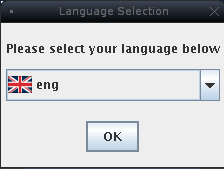
\includegraphics[width=5cm]{../image/LangChoice.png}
	\caption{Exemple de choix de langue avec IzPack}
\end{figure}

\subsubsection{Installation automatique}
A la fin de l'installation, il est possible de générer un script d'installation automatique. Ce script permet de reproduire l'installation réalisée sur d'autres machines.
\begin{figure}[H]
	\centering
	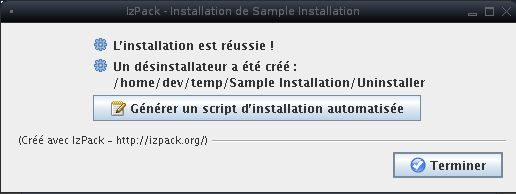
\includegraphics[width=12cm]{../image/SaveInstallXML.png}
	\caption{Fin d'installation, enregistrement du script d'installation automatisee}
\end{figure}

\subsection{Popularité}
Izpack est utilisé dans de grand projets comme Jboss, Xwiki, Glassfish... A l'heure actuelle, les téléchargements mensuels s'élèvent a 25.000.
% Image des telechargement?


 %---------------------------------------------------------
\section{Architecture}
\subsection{Architecture globale}
Globalement, Izpack possède 2 composants, le compilateur qui va gérer la création de l'installeur et l'installeur.
\subsection{Compilateur}
Le compilateur package l'ensemble des fichiers nécessaires dans un seul fichier jar. Selon la description de l'installation, il va incorporer les panels nécessaires au lancement de celle-ci. Cette partie est utilise par le developpeur qui souhaite creer un installeur.
\subsection{Installeur}
La partie installation concerne toute la logique et la présentation du processus d'installation. Cette partie sera executer par un utilisateur souhaitant installer le logiciel.
\subsubsection{Exemples de panels}
Chaque ecran que verra l'utilisateur est decrit par un panel.
Il existe de nombreux types de panels : des panel pour accueillir l'utilisateur et lui afficher des informations (HelloPanel et HTMLInfoPanel), d'autres pour demander à l'utilisateur des informations (UserInputPanel), etc.
Il existe aussi des panels plus spécialisés. Ainsi, CompilePanel permet de compiler du code java, et ProcessPanel permet de lancer des programmes après l'installation.

% screenshot de panels si on a du temps / de la place

 %---------------------------------------------------------
\section{Exemples d'installation}
De nombreux exemples complexes existent, par exemple l'installeur de IzPack, celui de Glassfish, etc. Pour illustrer simplement l'utilisation de IzPack, utilisons plutôt le petit exemple fourni avec le code de l'application.

\subsection{Description du xml}

% un peu porc comme méthode, copier/coller une partie du xml...
% mais je ne vois pas comment présenter ce xml
% et puis ça suffira, au moins pour un premier jet

Ce xml (install.xml) décrit complètement l'installation.
Une balise \verb|info| permet de définir les informations concernant l'application : 
\begin{lstlisting}[language=xml]
<info>
	<appname>Sample Installation</appname>
	<appversion>1.4 beta 666</appversion>
	...
</info>
\end{lstlisting}
Une autre balise, \verb|guipref| permet de définir quelques propriétés de la fenêtre de l'installeur :
\begin{lstlisting}[language=xml]
<guiprefs width="640" height="480" resizable="yes"/>
\end{lstlisting}
Les langues sont définies par la balise \verb|locale| :
\begin{lstlisting}
<locale>
	<langpack iso3="eng"/>
	<langpack iso3="fra"/>
</locale>
\end{lstlisting}
Des fichiers externes nécessaires à l'installation peuvent être définis par la balise \verb|resources| :

\begin{lstlisting}[language=xml]
<resources>
	<res id="LicencePanel.licence" src="Licence.txt"/>
</resources>
\end{lstlisting}
Les panels visibles par l'utilisateur sont décrits dans la balise \verb|panels| :
\begin{lstlisting}[language=xml]
<panels>
	<panel classname="HelloPanel"/>
	...
	<panel classname="FinishPanel"/>
</panels>
\end{lstlisting}
Enfin la balise \verb|packs| contient la description des packs (les differentes parties, optionnelles ou non, de l'application) a installer.
\begin{lstlisting}[language=xml]
<packs>
	<pack name="Base" required="yes">
		<description>The base files</description>
		<file src="Readme.txt" targetdir="$INSTALL_PATH"/>
		...
	</pack>
	<pack name="Docs" required="no">
		...
	</pack>
	...
</packs>
\end{lstlisting}
Bien sûr d'autres options existent, mais celles présentées ici suffisent à créer notre installeur.
\subsection{Génération du jar}
Pour générer notre installeur, il suffit d'avoir de lancer la commande suivante : (l'executable \verb|compile| provient de IzPack)
\begin{verbatim}
	compile install.xml
\end{verbatim}
Cette exécution va produire un fichier install.jar : notre installeur.
\subsection{Installation}
Il suffit désormais de lancer le jar pour installer notre application.
\begin{figure}[H]
	\centering
	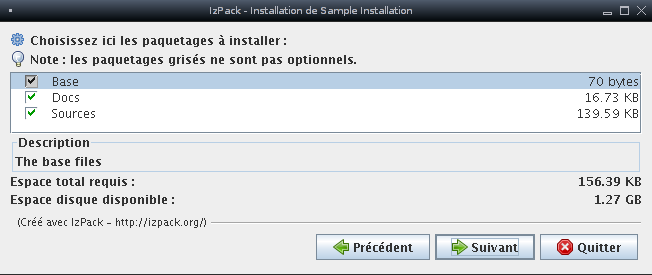
\includegraphics[width=15cm]{../image/installSample.png}
	% installSample.png: 652x275 pixel, 72dpi, 23.00x9.70 cm, bb=0 0 652 275
	\caption{Exemple d'installation avec IzPack}
\end{figure}

\subsection{Installation automatique}
En lancant l'installeur avec un script d'installation automatisee en parametre, l'installation est rejouee a l'identique automatiquement.

 %---------------------------------------------------------
\section{Problèmes actuels}
IzPack possède, comme tout logiciel, des bugs potentiels ou des améliorations à effectuer.
Heureusement, sa licence open-source permet à tout développeur d'apporter ses contributions.

\subsection{Nanoxml}
Une amélioration possible concerne la gestion des fichiers XML, qui ont une grande importance dans IzPack.
Pour lire/écrire des fichiers XML, IzPack se base sur une librairie, nanoXML. Cette librairie n'est malheureusement plus mise à jour (la dernière mise à jour date de 2003) et possède encore quelques bugs.
De plus, les versions récentes de l'environnement java (JRE) possèdent de base tout ce qu'il faut pour gérer le xml.
Se débarasser de la dépendance à nanoXML et se reposer uniquement sur la JRE permet donc non seulement de rendre la gestion des XML plus sûre et robuste, mais également de diminuer la taille de l'installeur généré.
%---------------------------------------
\renewcommand{\chaptermark}[1]{\markboth{\chaptername~\thechapter{} : #1}{}} \renewcommand{\sectionmark}[1]{\markright{\thesection{} #1}}
\chapter{IzPack}
\pagestyle{plain}
 %---------------------------------------------------------
\section{Description}
IzPack est un générateur d'installeur d'application open-source crée en 2001 par Julien Ponge.
\subsection{Générateur d'installeur}
A partir d'une application cree, Izpack est capable de generer un installateur. Cet installateur pourra etre utilise pour deployer l'application sur n'importe quelle machine. L'interet d'Izpack reside dans le fait que creer un installeur est souvent laborieux et n'apporte que peu de plus-value au programme. Izpack propose une solution pour creer cet installeur de maniere simple et universelle. 

Tout type de programme peut etre package, que ce soit une application C++, Java...
\subsection{Open-source}
Izpack est sous license Apache 2. Cette license permet l'acces au code source et l'utilisation du logiciel. Il est tout a fait possible de l'utiliser pour une application commerciale voire meme, de modifier les sources pour correspondre a ses besoins. Une importante communaute s'est regroupee autour de ce projet ce qui a permit son evolution jusqu'a maintenant. Si un developpeur apporte des modifications utiles, il est encourage a en faire profiter la communaute, mais ce n'est pas une obligation.

\subsection{Fonctionnalités}
Izpack est un systeme modulaire, il possède de nombreuses fonctionnalités pour creer un installeur adapte a chacun.
\subsubsection{Multi-plateforme}
L'installeur generee par Izpack est un jar (java archive). Il suffit donc que la machine ait un machine virtuelle pour pouvoir lancer l'installation, indépendamment de la plateforme et du système d'exploitation. Il est neanmoins possibles de faire des traitements specifiques a certaines plateforme ou de convertir l'installeur pour etre specifique a une plateforme. 
\subsubsection{Personnalisation}
Izpack propose un ensemble de panels qui vont constituer l'installateur graphique. Chaque panels remplit une fonction specifique. L'aspect global et celui des panels est personnalisable par l'utilisateur via le descripteur XML.

\subsubsection{Internationalisation}
Izpack supporte la création d'installeur multilangues. Pour la localisation, tout repose sur des fichiers XML. Si une langue n'existe pas, il suffit de traduire les phrases/mots dans un fichier xml a utiliser lors de la creation de l'installeur.

\begin{figure}[H]
	\centering
	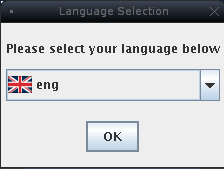
\includegraphics[width=5cm]{../image/LangChoice.png}
	\caption{Exemple de choix de langue avec IzPack}
\end{figure}

\subsubsection{Installation automatique}
A la fin de l'installation, il est possible de générer un script d'installation automatique. Ce script permet de reproduire l'installation réalisée sur d'autres machines.
\begin{figure}[H]
	\centering
	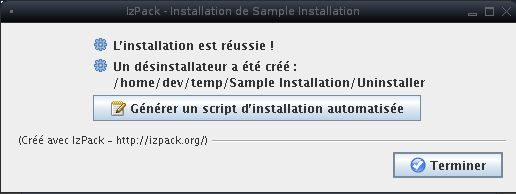
\includegraphics[width=12cm]{../image/SaveInstallXML.png}
	\caption{Fin d'installation, enregistrement du script d'installation automatisee}
\end{figure}

\subsection{Popularité}
Izpack est utilisé dans de grand projets comme Jboss, Xwiki, Glassfish... A l'heure actuelle, les téléchargements mensuels s'élèvent a 25.000.
% Image des telechargement?


 %---------------------------------------------------------
\section{Architecture}
\subsection{Architecture globale}
Globalement, Izpack possède 2 composants, le compilateur qui va gérer la création de l'installeur et l'installeur.
\subsection{Compilateur}
Le compilateur package l'ensemble des fichiers nécessaires dans un seul fichier jar. Selon la description de l'installation, il va incorporer les panels nécessaires au lancement de celle-ci. Cette partie est utilise par le developpeur qui souhaite creer un installeur.
\subsection{Installeur}
La partie installation concerne toute la logique et la présentation du processus d'installation. Cette partie sera executer par un utilisateur souhaitant installer le logiciel.
\subsubsection{Exemples de panels}
Chaque ecran que verra l'utilisateur est decrit par un panel.
Il existe de nombreux types de panels : des panel pour accueillir l'utilisateur et lui afficher des informations (HelloPanel et HTMLInfoPanel), d'autres pour demander à l'utilisateur des informations (UserInputPanel), etc.
Il existe aussi des panels plus spécialisés. Ainsi, CompilePanel permet de compiler du code java, et ProcessPanel permet de lancer des programmes après l'installation.

% screenshot de panels si on a du temps / de la place

 %---------------------------------------------------------
\section{Exemples d'installation}
De nombreux exemples complexes existent, par exemple l'installeur de IzPack, celui de Glassfish, etc. Pour illustrer simplement l'utilisation de IzPack, utilisons plutôt le petit exemple fourni avec le code de l'application.

\subsection{Description du xml}

% un peu porc comme méthode, copier/coller une partie du xml...
% mais je ne vois pas comment présenter ce xml
% et puis ça suffira, au moins pour un premier jet

Ce xml (install.xml) décrit complètement l'installation.
Une balise \verb|info| permet de définir les informations concernant l'application : 
\begin{lstlisting}[language=xml]
<info>
	<appname>Sample Installation</appname>
	<appversion>1.4 beta 666</appversion>
	...
</info>
\end{lstlisting}
Une autre balise, \verb|guipref| permet de définir quelques propriétés de la fenêtre de l'installeur :
\begin{lstlisting}[language=xml]
<guiprefs width="640" height="480" resizable="yes"/>
\end{lstlisting}
Les langues sont définies par la balise \verb|locale| :
\begin{lstlisting}
<locale>
	<langpack iso3="eng"/>
	<langpack iso3="fra"/>
</locale>
\end{lstlisting}
Des fichiers externes nécessaires à l'installation peuvent être définis par la balise \verb|resources| :

\begin{lstlisting}[language=xml]
<resources>
	<res id="LicencePanel.licence" src="Licence.txt"/>
</resources>
\end{lstlisting}
Les panels visibles par l'utilisateur sont décrits dans la balise \verb|panels| :
\begin{lstlisting}[language=xml]
<panels>
	<panel classname="HelloPanel"/>
	...
	<panel classname="FinishPanel"/>
</panels>
\end{lstlisting}
Enfin la balise \verb|packs| contient la description des packs (les differentes parties, optionnelles ou non, de l'application) a installer.
\begin{lstlisting}[language=xml]
<packs>
	<pack name="Base" required="yes">
		<description>The base files</description>
		<file src="Readme.txt" targetdir="$INSTALL_PATH"/>
		...
	</pack>
	<pack name="Docs" required="no">
		...
	</pack>
	...
</packs>
\end{lstlisting}
Bien sûr d'autres options existent, mais celles présentées ici suffisent à créer notre installeur.
\subsection{Génération du jar}
Pour générer notre installeur, il suffit d'avoir de lancer la commande suivante : (l'executable \verb|compile| provient de IzPack)
\begin{verbatim}
	compile install.xml
\end{verbatim}
Cette exécution va produire un fichier install.jar : notre installeur.
\subsection{Installation}
Il suffit désormais de lancer le jar pour installer notre application.
\begin{figure}[H]
	\centering
	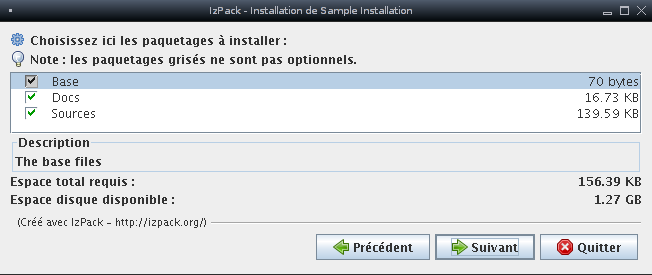
\includegraphics[width=15cm]{../image/installSample.png}
	% installSample.png: 652x275 pixel, 72dpi, 23.00x9.70 cm, bb=0 0 652 275
	\caption{Exemple d'installation avec IzPack}
\end{figure}

\subsection{Installation automatique}
En lancant l'installeur avec un script d'installation automatisee en parametre, l'installation est rejouee a l'identique automatiquement.

 %---------------------------------------------------------
\section{Problèmes actuels}
IzPack possède, comme tout logiciel, des bugs potentiels ou des améliorations à effectuer.
Heureusement, sa licence open-source permet à tout développeur d'apporter ses contributions.

\subsection{Nanoxml}
Une amélioration possible concerne la gestion des fichiers XML, qui ont une grande importance dans IzPack.
Pour lire/écrire des fichiers XML, IzPack se base sur une librairie, nanoXML. Cette librairie n'est malheureusement plus mise à jour (la dernière mise à jour date de 2003) et possède encore quelques bugs.
De plus, les versions récentes de l'environnement java (JRE) possèdent de base tout ce qu'il faut pour gérer le xml.
Se débarasser de la dépendance à nanoXML et se reposer uniquement sur la JRE permet donc non seulement de rendre la gestion des XML plus sûre et robuste, mais également de diminuer la taille de l'installeur généré.
%---------------------------------------
\chapter{Méthodes de travail}
\subsection{Utilisation de NanoXML}
\begin{frame}\frametitle{Utilisation de NanoXML}
Utilisations principales :
\begin{itemize}
	\item XMLParser : 23 fois
	\item XMLWriter : 8 fois
	\item XMLElement : 499 fois
\end{itemize}
\end{frame}
%------------------------------------------------------------------------------
\subsection{Solutions possibles}
\begin{frame}\frametitle{Solutions possibles}
\begin{minipage}[c]{.46\linewidth}
\begin{beamerboxesrounded}[shadow=true]{Modification du code}
\begin{itemize}
	\item Améliorer NanoXML
	\item Réécrire un parseur
\end{itemize}
\end{beamerboxesrounded}
\end{minipage}
\hfill
\begin{minipage}[c]{.46\linewidth}
\begin{beamerboxesrounded}[shadow=true]{Changement de langage}
\begin{itemize}
	\item Abandonner le XML pour un autre langage
\end{itemize}
\end{beamerboxesrounded}
\end{minipage}
\vfill
\hfil
\begin{minipage}[c]{.8\linewidth}
\begin{beamerboxesrounded}[shadow=true]{Changement de librairie}
\begin{itemize}
	\item Librairie externe (Xerces, JDOM, ...)
	\item Librairie interne (JAXP)
\end{itemize}
\end{beamerboxesrounded}
\end{minipage}
\end{frame}
%------------------------------------------------------------------------------
\subsection{Pertinence de la solution}
\begin{frame}\frametitle{Critères de sélection}
Critères importants dans IzPack :
\begin{itemize}
	\item Taille de la librairie
	\item Transition
	\item Performances
	\item Évolution
\end{itemize}
\end{frame}
%------------------------------------------------------------------------------
\begin{frame}\frametitle{Solution la plus adaptée}
JAXP :
\begin{itemize}
	\item Intégrée à la JRE
	\item Spécification DOM
	\item Évolution
\end{itemize}
\end{frame}
%------------------------------------------------------------------------------

%---------------------------------------
\chapter{Travail réalisé}
Le projet étant open-source et actif, il évolue sans cesse. La partie sur laquelle nous avons travaillé est relativement stable mais son utilisation peut varier dans le code. Nous allons voir la portée de l'utilisation de nanoXml, comment il est utilisé et enfin la solution apportée.

% -> Utilisation intensive de XML
% -> Philosophie de nanoXml et de DOM differente
% -> -> DOM : Tout est noeud
% -> -> NanoXml : Base sur les tags (elements)
\section{Etude de Nanoxml}
Comme nous avons pu le voir, IzPack utilise intensément des fichiers XML pour la génération d'installations.
En effet, les fichiers XML présentent l'avantage d'être lisible, écrivable a la main et traitables.
Pour traiter ces fichiers, une librairie a été utilisée, il s'agit de NanoXml.
\subsection{Le projet NanoXml}
NanoXml est une librairie java open-source de gestion de Xml.
Elle présente la particularité d'être légère (108Ko). 
Il est possible, grâce a cette librairie, d'écrire ou de parser des fichiers Xml.
Une fois le fichier parsé, on récupère en mémoire la structure de l'arbre Xml qui peut alors être exploité.
Le choix de cette librairie a été faite au commencement de Izpack a cause de sa taille.
En effet, il est important que le la partie installeur ne surcharge pas excessivement sur le logiciel à installer.

Cependant ce projet n'est plus mis à jour depuis 7 ans, et des bugs ont été découverts.
Entre temps, java a ajouté a sa JRE (depuis la version 1.4) tout ce qu'il faut pour gérer le xml.
Il devenait intéressant de remplacer NanoXml par Jaxp (Java API for XML Processing), la librairie fournie par la machine virtuelle.
\subsection{Les différents composants de NanoXml}
On trouve différents éléments dans NanoXml.
\subsubsection{StdXMLParser}
Le parser permet de créer un arbre logique représentant le fichier xml qui lui a été passé.
Il est systématiquement utilisé au moment de la lecture du fichier afin de récupérer l'arbre.
\subsubsection{StdXMLWriter}
Le XMLWriter permet d'écrire des fichiers XML.
Il reproduit, à partir d'un XMLElement, le fichier XML correspondant.
Il n'est utilisé que pour générer un xml temporaire lors de la compilation ou pour écrire le xml d'installation automatique.
\subsubsection{XMLElement}
Le XMLElement représente un élément logique du xml en mémoire. Par exemple :
\begin{lstlisting}[language=xml]
<root>
	<child>
		content
	</child>
</root>
\end{lstlisting}
En parsant un fichier contenant ce Xml, on obtient un XMLElement nommé root qui possède 1 enfant, \verb|child|. Son enfant est un XMLElement dont le contenu est ``content''.

L'arborescence du XML est donc réalisé par un ensemble de XMLElement.
L'interface de XMLElement permet de récupérer la liste des enfants, le contenu, rechercher un enfant par son nom, retirer un enfant, ajouter un enfant ou modifier le contenu.
Il s'agit de loin de la classe la plus utilisée de la librairie NanoXml dans Izpack.
En effet, on ne comptait pas moins de 499 utilisations au commencement de ce projet.
\subsection{Utilisation typique dans Izpack}
\subsubsection{Parse de fichier}
Le parse du fichier est exécuté pour récupérer le XML.
\begin{lstlisting}
StdXMLParser parser = new StdXMLParser();
parser.setBuilder(XMLBuilderFactory.createXMLBuilder());
parser.setReader(new StdXMLReader(in));
parser.setValidator(new NonValidator());
// We get the data
XMLElement data = (XMLElement) parser.parse();
\end{lstlisting}
Avec cet exemple, on crée les objets nécessaires au parse d'un fichier, et on récupère dans \verb|data| la racine de l'arborescence du xml chargé en mémoire.
\subsubsection{Écriture d'un xml}
\begin{lstlisting}
XMLWriter writer = new XMLWriter(out);
...
writer.write(xmlElement);
\end{lstlisting}
Le XMLWriter prend un OutputStream à sa contruction.
On peut donc écrire un Xml dans tout type de flux de sortie. 
Une fois le XMLWriter instancié, il suffit de lui passer le \verb|xmlElement| représentant la racine de l'arborescence que l'on veut écrire.
\subsubsection{Utilisation de XMLElement}
La manipulation d'un XMLElement se fait avec ses méthodes :
\begin{itemize}
	\item get/setAttribute pour gérer les attributs du noeud
	\item get/setContent pour gérer le contenu
	\item add/removeChild pour gérer les noeuds fils
	\item etc
\end{itemize}
Voici un exemple d'utilisation :
% TODO : avoir un exemple plus clair/concis
\begin{lstlisting}
XMLElement root;
//...
Iterator<XMLElement> iter = root.getChildrenNamed("parsable").iterator();
while (iter.hasNext())
{
	XMLElement p = iter.next();
	String target = requireAttribute(p, "targetfile");
	String type = p.getAttribute("type", "plain");
	//...
}
\end{lstlisting}
\section{Etude Jaxp}
Jaxp, le processeur Xml de Sun, respecte les normes W3C.
Il y a deux manières d'exploiter les XML avec Jaxp, soit en utilisant le parseur SAX, soit en utilisant le parseur DOM.
\subsection{SAX}
SAX (Simple API for Xml) est une API pour parser les XML.
Cette API possède la particularité de procéder par évènement.
C'est à dire que le parser va lire le fichier ligne par ligne et envoyer un évènement pour chaque élément particulier qu'il rencontre.

Des évènements sont lancés des que le parse rencontre des commentaires, du texte, des éléments...
L'avantages de cette API est l'utilisation mémoire faible, puisque le xml n'est pas mis en mémoire mais lu et traité au fur et à mesure, il permet de traiter sans problème les fichiers importants.
En contrepartie, le traitement et la manipulation du xml est plus difficile.
\subsection{DOM}
L'interface DOM (Document Object Model) de Jaxp propose de mettre en mémoire le xml et offre une interaction basée sur des noeuds (node en anglais).
En DOM tout est noeud, les commentaires, le texte ou les éléments sont représentés par des noeuds.
Le xml est est représenté par une arborescence de noeuds.
Des sous-classes spécialisent ces noeuds comme \verb|Comment|, \verb|Element| ou \verb|Text|.

La manipulation des éléments du xml se fait grâce aux nodes.
Il est possible de récupérer le voisin d'une node, d'enlever ou d'ajouter un enfant et de récupérer ou de modifier le contenu.
%--------------------------------------------------------------------------
\section{Élaboration de la solution}
Notre travail a été de chercher une solution pour permettre de remplacer de NanoXml et de l'appliquer au projet.
Cependant, ils y avaient plusieurs problèmes à cela.
\subsection{Les différences entre Jaxp et NanoXml}
Comme nous avons vu précédemment, les deux API ne proposent pas la même approche pour le traitement des fichiers xml.
Nous avons choisi d'utiliser l'interface DOM vu que les avantages de SAX ne sont pas nécessaires et qu'il était peu concevable de traiter les XML avec SAX dans IzPack.
De plus, NanoXml et DOM ont une représentation similaire du xml.
Nous allons donc comparer l'interface DOM et NanoXml pour déterminer la meilleure approche a prendre.
\subsubsection{Manipulation du XML}
La principale différence vient de l'élément atomique : le noeud de DOM ne représente pas la même notion que l'élément de nanoXML.
Dès lors, la manipulation des voisins, enfants, etc doit être adapté.
\begin{lstlisting}[language=xml]
<!-- commentaire -->
<root>
	<noeud1>text</noeud1>
</root>
\end{lstlisting}
Dans ce morceau de xml, nanoXML comptera 1 enfant à l'élément \verb|root| : \verb|noeud1|.
DOM comptera 3 noeuds : du texte (le retour à la ligne et la tabulation), \verb|noeud1| et à nouveau du texte (un retour à la ligne).

DOM possède néanmoins une interface dérivant de \verb|Node| : \verb|Element|, qui est très similaire à la classe \verb|XMLElement| de nanoXML.
\subsubsection{Contenu textuel du noeud}
NanoXml propose une méthode pour récupérer le contenu textuel d'un noeud : \verb|getContent()|.
DOM propose une méthode semblant équivalente : \verb|getNodeValue()|.
Cependant, le comportement de ces deux méthodes est complètement différent.
Prenons par exemple le code XML suivant :
\begin{lstlisting}[language=xml]
<testElement>
	foobar
</testElement>
\end{lstlisting}
Placé sur l'élément \verb|testElement|, \verb|getContent()| renvoie le texte (avec des retours à la ligne) ``foobar'' tandis que \verb|getNodeValue()| renvoie \verb|null| (il faut utiliser cette méthode sur le fils, le texte, pour avoir exactement le même résultat).
Malheureusement, le comportement de NanoXml devient erratique avec les éléments CDATA et le texte :
\begin{lstlisting}[language=xml]
<testElement>
	<![CDATA[ be <bold> ]]>
</testElement>
\end{lstlisting}
NanoXml renverra le résultat suivant, sans retour à la ligne :
\begin{verbatim}
' be <bold> '
\end{verbatim}
La concaténation des valeurs des fils donne, avec DOM :
\begin{verbatim}
'
         be <bold> 
'
\end{verbatim}
On voit ici un comportement peu cohérent (NanoXml ignore dans certains cas les caractères blancs), qu'il faudra gérer.

\subsection{Solutions possibles}
Pour remplacer NanoXml, plusieurs approches étaient possibles.

\subsubsection{Remplacer les appels individuellement}
La première solution, bête et méchante, est de remplacer systématiquement les appels à NanoXml par des appels à Jaxp.
Cependant, cette solution a des inconvénients évidents :
\begin{description}
\item[La duplication de la logique] Tout le code nécessaire à l'utilisation du parseur ou du Node est réparti et dupliqué dans tout le programme.
C'est d'abord une infraction au principe DRY (don't repeat yourself) et rend le code difficile a maintenir.
Les bugs sont plus difficiles à cibler et la correction doit se faire sur toutes les replications.
\item[Les difficultés de tester la solution] Un autre problème et le test de cette solution.
Il faut en théorie passer par toutes les utilisations des appels pour tester correctement la solution. Cette contrainte est difficilement réalisable.
\item[La pénibilite de la tâche] Remplacer chacun des nombreux appels à NanoXml par un appel Jaxp est très laborieux.
\end{description}
\subsubsection{Centraliser la logique de modification}
L'autre solution possible est de centraliser toute la logique de traduction dans des classes dédiées.
Ces classes vont copier les interfaces de NanoXml mais vont générer en réalité des appels à Jaxp. 
C'est le principe du design pattern adaptateur.

Cela présente plusieurs avantages.
\begin{description}
\item[Centralisation de la logique] Toute la logique de traduction est centralisée en un endroit. Il est facile de corriger les éventuelles erreurs.
\item[Rapidité de déploiement] L'adaptateur présente l'avantage de ne pas changer la logique d'utilisation. Les changements d'appels se résument a changer le nom de la classe et les imports.
\end{description}
\subsection{Création de l'adaptateur}
Nous avons donc choisi la solution de l'adaptateur pour notre problème. Pour cela, nous avons procéder en plusieurs étapes.
\subsection{Repérer les utilisations des classes de NanoXml}
Dans un premier temps, nous avons repérer les classes utilisées par Izpack et les méthodes utilisées de ces classes.
Nous avons réduits l'utilisation de NanoXml à 3 classes : \verb|StdXMLParser|, \verb|StdXMLWriter| et \verb|XMLElement|.
\subsubsection{StdXMLParser et StdXMLWriter}
Les classes \verb|StdXMLParser| et \verb|StdXMLWriter| sont utilisées avec parcimonie.
On compte une trentaine d'utilisations pour \verb|StdXMLParser| et 8 utilisations pour \verb|StdXMLWriter|.
Modifier l'interface pour ces deux classes n'étaient pas un problème.
Ces deux classes ont donc été remplacées par 2 nouvelles classes réalisant les mêmes fonctionnalités avec des prototypes différents.

Nous avons créé les interfaces \verb|IXmlParser| et \verb|IXmlWriter| ainsi que leurs implémentations.
Ce ne sont pas des adaptateurs de NanoXml étant donnés qu'elles ne recopient pas l'interface de NanoXml et elles ne sont pas indispensables.
Cependant, elles permettent de simplifier l'utilisation de Jaxp et de factoriser le code sur un endroit.
\subsubsection{XMLElement}
\verb|XMLElement| ne présente pas d'interface et est utilisé systématiquement quand il y a du XML à traiter.
Il était donc impensable de traiter et remplacer toutes les utilisations de XMLElement par des appels à Jaxp étant donné son nombre d'utilisation (499 utilisations).
Nous avons donc concentré nos efforts sur cette classe et appliquer le pattern adaptateur dessus.
Nous avons pour cela procédé en plusieurs étapes.

Dans un premier temps, nous avons extrait l'interface de \verb|XMLElement| avec toutes les méthodes utilisées par Izpack.
\begin{figure}[H]
	\centering
	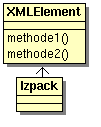
\includegraphics[width=0.15\textwidth]{../image/sol_casInitial.png}
	\hfil
	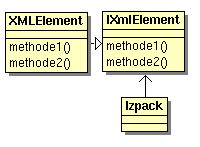
\includegraphics[width=0.3\textwidth]{../image/sol_extractionInterface.png}
	\caption{Extraction de l'interface}
\end{figure}
Nous avons ensuite créé l'implémentation de l'adaptateur respectant l'interface.
Izpack utilise alors la même interface mais notre implémentation était utilisé.
\begin{figure}[H]
	\centering
	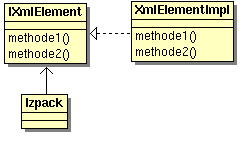
\includegraphics[width=0.4\textwidth]{../image/sol_implementation.png}
	\caption{Implémentation de l'adaptateur}
\end{figure}
Il suffit alors de supprimer NanoXml, ses utilisations ayant été remplacés par notre implémentation.
\subsection{Implémentation de Xinclude}
Avec NanoXml, la balise \verb|xinclude| permet d'inclure un fichier xml externe.
Ainsi, on peut utiliser un xml très succinct (et donc facilement lisible/compréhensible) qui inclut d'autres fichiers xml décrivant uniquement certaines parties de l'installation.
Cette fonctionnalité, absente de nanoXML, avait été mise en place en modifiant directement le code de son parseur.

Xinclude est présente dans les normes W3C et Jaxp l'intègre dans son implémentation.
Pour que Jaxp prenne en compte les balises Xinclude, il faut que le parser prenne en compte les espaces de nommage (namespaces) XML.
En effet, le Xinclude appartient au namespace \verb|xi|.
Il faut donc utiliser la balise \verb|<xi:include/>| au lieu de \verb|<xinclude/>|.
Le simple fait de rendre le parser namepaceAware permet d'utiliser la fonctionnalité Xinclude.
\subsection{Implémentation de Xfragment}
La fonctionnalité Xfragment permet principalement d'ajouter des éléments sans racines avec Xinclude.
C'est à dire qu'au contenu du xml à ajouter, on va retirer les noeuds \verb|<xfragment>|.
Par exemple:
\begin{lstlisting}[language=xml]
<xfragment>
<root1>
	<noeud1>text</noeud1>
</root1>
<root2>
	<noeud1>text</noeud1>
</root2>
</xfragment>
\end{lstlisting}
Si ce xml est inclus, 2 éléments, \verb|<root1>| et \verb|<root2>| seront ajouté à l'emplacement du Xinclude.
Sans le xfragment, le Xml ne serait pas valide (plusieurs éléments racine) et il y aurait erreur au moment du parse.
Le Xfragment agit ici comme conteneur temporaire d'éléments.

Cette fonctionnalité a été rajouté a NanoXml et il était nécessaire de la conserver.
Cependant, elle ne fait pas partie des spécifications W3C et le parseur n'offre pas de base cette fonctionnalité.
Il a fallut trouver une solution pour implémenter cette fonctionnalité.
\subsubsection{Première solution, manipulation du DOM}
Une première solution est de modifier le DOM obtenu après le parse du XML. 
Il faudrait chercher les noeuds nommer Xfragment et les supprimer.
Cependant, la suppression d'un noeud en DOM entraîne la suppression de tout les éléments qu'il contient.
Il faudrait donc au préalable sauvegarder le contenu, supprimer l'élément et restaurer le contenu sauvegardé.
\subsubsection{Deuxième solution, surcharge du parseur}
Une autre solution est de procéder de la même manière que pour ce qui a été fait pour NanoXml.
C'est à dire de modifier le parseur pour traiter les xfragment de manière spécifique.
Cependant, cette solution, possible sous NanoXml, est difficilement réalisable sur Jaxp. 
En effet, les appels du parseur sont transmis vers des classes internes et difficilement manipulables.
\subsubsection{Troisième solution, transformation XSL}
La troisième solution a été proposé par Matthew Fudge, la personne ayant rajouté la gestion des Xfragment et Xinclude dans NanoXml pour IzPack.
Elle consiste à transformer l'arbre xml obtenu après le parse grâce à une transformation XSL (Extensible Stylesheet Language).
Les transformations XSL permettent de définir des règles de modification d'un XML et se présente lui-même sous la forme d'un XML.
Elles permettent de modifier facilement des XML de manière simple.
Elle convenait parfaitement à notre problème.
La feuille de style utilisé est la suivante :
\begin{lstlisting}[language=xml]
<xsl:stylesheet 
	xmlns:xsl='http://www.w3.org/1999/XSL/Transform' version='1.0'>
    <!-- tous les elements -->
    <xsl:template match="*">
        <xsl:copy>
            <xsl:copy-of select="@*"/>
            <xsl:apply-templates/>
        </xsl:copy>
    </xsl:template>a

    <!-- les elements xfragment -->
    <xsl:template match="xfragment">
        <xsl:apply-templates/>
    </xsl:template>
</xsl:stylesheet>
\end{lstlisting}

La règle appliquée sur un élément est la plus spécifique.
Ici, pour tout les éléments, on recopie l'élément.
Dans le cas du xfragment, on omet la copie.
Au final, le xfragment est supprimé du XML ce qui est le but recherché.
\subsection{Numéro de ligne}
Une fonctionnalité de nanoXML est la gestion des numéros de lignes. 
Lors qu'une incohérence est détectée dans un XML lu, IzPack prévient l'utilisateur de l'erreur, et indique le numéro de la ligne responsable dans le xml.

Du point de vue de DOM, les numéros de lignes n'ont pas de signification : une fois le fichier XML parsé, seul l'arbre DOM construit en mémoire importe. 
Cet arbre, réécrit dans un fichier ne correspondra pas forcèment (pour les numéros de lignes, l'indentation, etc) au fichier de départ, sans parler des ajouts/suppressions/modifications de noeuds.

Au contraire, pour SAX, les numéros de lignes sont obtenues facilement.
Dans ce cas là, il est utile de savoir à quel endroit on se trouve dans le document.

Afin d'obtenir les numéros de ligne dans un arbre DOM, les deux points de vue ont été utilisés grâce à un \verb|Transformer|.
Cet objet permet (entre autre) d'utiliser un parseur SAX pour remplir un arbre DOM.
Lors du parse SAX on retient les numéros de lignes, qui seront ajoutés aux bons éléments du DOM.
Ce nombre est stocké dans les ``user data'', ajoutés dans la version 3  de DOM pour stocker diverses informations supplémentaires dans un noeud.

\section{Application et tests}
Une fois la solution réalisée, nous l'avons soumis à un certain nombre de tests afin de la vérifier.
\subsection{Tests}
Afin d'avoir un comportement le plus fidèle possible à celui de NanoXML et assurer la fiabilité de la solution, de nombreux tests unitaires ont été écrits.
\subsubsection{Test unitaires de comparaison}
La solution a d'abord été élaborée de manière isolée.
Un projet indépendant contenant NanoXml à été créé. 
C'est sur ce projet que nous avons travaillé et développer notre adaptateur.
Nous avons alors réalisé une batterie de tests couvrant toutes les méthodes de l'interface extraites et de très nombreux cas.
Ces tests unitaires effectuent des actions identiques avec notre adaptateur et NanoXML, et comparent les résultats.

Prenons l'exemple de la méthode \verb|getName()|. Le même fichier Xml est parsé par les 2 librairies.
Un parcours récursif de l'arbre XML est effectué sur les 2 arbres en mémoire.
Pour chaque élément, on compare le résultat de la méthode \verb|getName()| sur l'élément courant : les retours doivent être toujours égaux.

Comme les méthodes de XMLElement sont souvent des récupérations d'informations de la même nature que getName(), nous avons généralisé ce test à ces méthodes.
Pour cela, une méthode se charge de parcourir de manière récursive l'arbre et d'invoquer la méthode à tester en comparant leurs résultats.
Ceci nous a permis de nous assurer du comportement de l'adaptateur et de déceler des anomalies sur NanoXml.

En couvrant la quasi totalité des méthodes utilisées dans IzPack avec de nombreux cas d'utilisation, nous avons pu nous assurer du respect du comportement de notre adaptateur.
\subsubsection{Les tests unitaires sur Xinclude et Xfragment}
Avec l'ajout des fonctionnalités XInclude et XFragment à NanoXml, une batterie de test unitaires a été fournies.
Nous avons donc repris ces tests et nous les avons intégrés aux tests de l'adaptateur.
\subsubsection{Les tests unitaires classiques}
Nous avons créé une batterie de tests unitaires classiques pour notre adaptateur.
Ils s'assurent entre autre que le parse, l'exploitation de l'arbre en mémoire et l'écriture du Xml se font correctement.
\subsection{Intégration a IzPack}
L'intégration à IzPack de notre travail fut relativement aisée : les objets de NanoXml ont été remplacés par ceux de notre adapteur.
Les appels n'ont quasiment pas été changés, les méthodes exposées dans les deux cas étant les mêmes.
Cette intégration effectuée, nous avons pu commencer les tests sur application.
\subsubsection{Test fonctionnels}
Une phase de test fonctionnels a été réalisée pour tester l'intégrité de l'application après l'intégration de notre solution.
Ces tests sont des tests manuels sur les installations générés par Izpack.
Nous avons donc testé dans un premier temps l'application d'exemple fourni par Izpack.
Ces tests ont permis de faire ressortir quelques problèmes que nous avons pu régler rapidement.

Suite à cela, nous avons essayé de générer et lancer un installeur plus conséquent.
Nous avons pour cela utilisé l'installeur de Glassfish.
La génération et l'installation de glassfish s'est déroulé sans problème.
\subsubsection{Profiling}
Après la phase d'implémentation et de test, nous avons pu commencer une phase d'optimisation.
En utilisant YourKit, nous avons essayé de détecter les méthodes chronophages lors d'une installation et les modifier éventuellement.

Pour profiler l'application avec yourkit, il faut placer la librairie de yourkit dans le PATH. 
Une fois cette opération réalisée, il suffit de lancer l'application à profiler avec l'option \verb|-agentlib:yjpagent|.
Il est alors possible de connecter le profiler à l'application et lancer le profiling.

Le profiling lancé, nous utilisons l'application normalement. 
A la fin de l'exécution, une image de l'exécution(snapshot) est enregistrée qui peut être analysée après.
Cette image comporte toutes les informations du profiling comme la trace des appels, le temps passés dans chaque méthodes, le nombre d'appels aux méthodes, l'utilisation de la mémoire et du garbage collector à chaque moment de l'exécution...
Nous avons profilé deux version de l'installeur de Glassfish; l'un a été généré avec la version 4.2.1 de IzPack et l'autre avec la dernière version construite à partir du dépôt et comportant nos modifications.

Par exemple, on peut rechercher tout les appels à l'objet XmlElementImpl de notre adaptateur pour voir les différentes méthodes utilisées. Sur la figure~\ref{fig:yourkitXmlElement}, on peut voir que la méthode getAttribute() est utilisée majoritairement.
\begin{figure}[H]
	\centering
	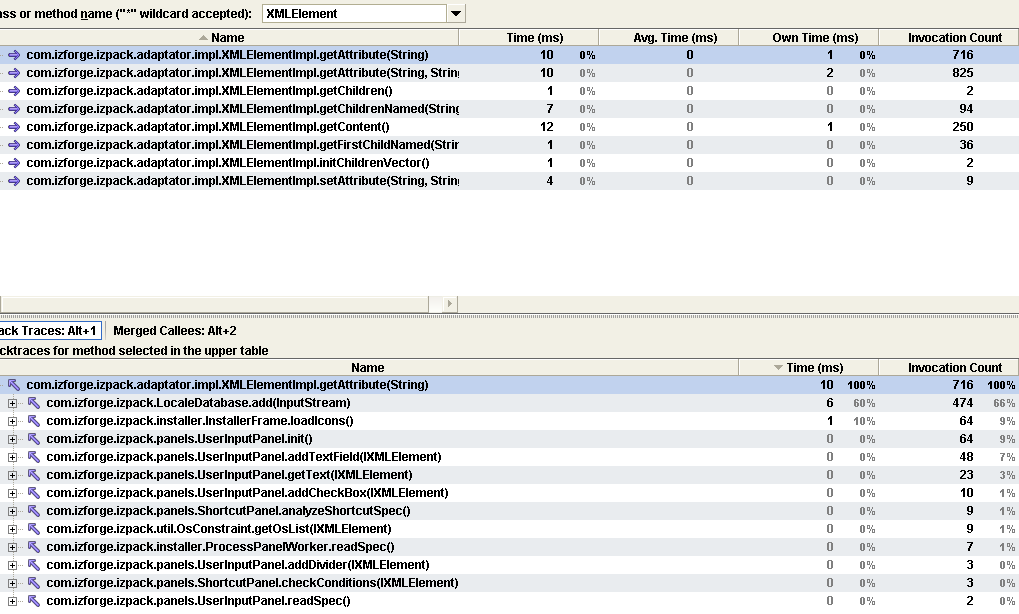
\includegraphics[width=1\textwidth]{../image/yourkitXmlElement.png}
	\caption{Trace des appels au XmlElement}
	\label{fig:yourkitXmlElement}
\end{figure}

On peut également comparer deux snapshots et obtenir la différence dans les temps d'exécution et les appels.
Sur la figure~\ref{fig:yourkitComparaison}, nous comparons les deux installeurs et filtrons les appels aux xmlElement.
On voit apparaître le XMLElement de NanoXml pour la version 4.2.1 et le XMLElementImpl de notre adaptateur.
On voit que les performances entre les deux sont sensiblement les mêmes, les gains possibles sont relativement faibles et peu d'optimisation ont été faites. 
\begin{figure}[H]
	\centering
	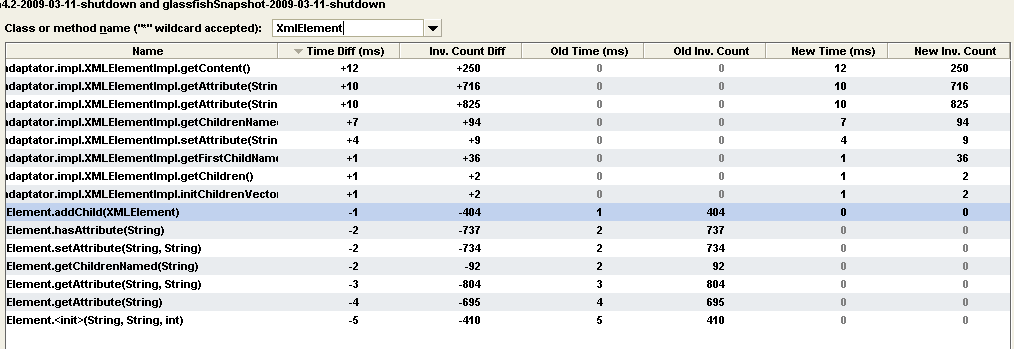
\includegraphics[width=1\textwidth]{../image/yourkitComparaison.png}
	\caption{Comparaison entre deux snapshots}
	\label{fig:yourkitComparaison}
\end{figure}
\section{Résultats}
Le principal but de notre projet a été de pouvoir abandonner NanoXml ce qui est chose faite.
De plus, l'intégration de notre solution a apporté un certain nombres d'avantages.
\subsection{Diminution de la taille des installeurs}
Tout d'abord, l'abandon de NanoXml diminue la taille de IzPack et des installeurs générés car cette librairie n'a plus besoin d'être présente dans les installeurs.
NanoXml pèse, une fois compilé, 116Ko.
Notre adaptateur pèse 44Ko.
Chaque installeur généré par Izpack perdra donc 72Ko.
Ce chiffre peut paraître faible mais si l'installeur est téléchargé 25000 fois sur le site officiel, presque 1800 Mo de bande passante sont économisés.
\subsection{Support de fonctionnalités XML}
Outre le fait d'avoir un parseur plus fiable et récent, un certain nombre de nouveautés ont été apportées.
\subsubsection{Support de la DTD}
Désormais les DTD (document de validation d'un xml) sont pris en charge.
\subsubsection{Support natif de Xinclude}
De plus, l'inclusion de fichiers xml dans d'autres est supporté nativement, sans avoir à modifier le code du parseur.
\subsection{Intégration dans la branche principale}
Régulièrement, nous synchronisions notre dépôt avec la branche principale pour prendre en compte les modifications qui ont été réalisées sur Izpack.
Cette synchronisation se passait généralement sans encombre grâce à Git, excepté quand les modifications concernaient la manipulation de XML et que les fichiers étaient conséquents (>3000 lignes).

Cette synchronisation régulière était en vue de préparer le merge vers sur la branche principale.
Ainsi, une fois notre solution achevée et testée, Julien Ponge a extrait un patch qui a été soumis à la communauté des développeurs d'Izpack.
Après quoi, les modifications ont été portées sur la branche principale et seront disponibles pour la prochaines version d'Izpack, la 4.3.
\section{Au delà du sujet}
Une fois l'objectif du projet atteint, nous avons décidé d'accepter l'offre de Julien Ponge en devenant contributeurs officiels du projet.
\subsection{Le projet Izpack}
Izpack est une communauté Open-Source, sa structure et son fonctionnement sont particuliers. 
Le projet est récemment passé sous CodeHaus. 
Des outils et des moyens de communications sont dédiées au projet.
\subsubsection{Codehaus}
CodeHaus est une fondation dédiée au développement de projets open-source.
A ce titre, elle propose une plateforme pour aider au développement de ces projets avec un certains nombre d'outils fournis par des sponsors.
Par exemple, Atlassian fournit pour les projets leur système de suivie de bug, JIRA, JetBrain fournit une licence IntelliJ, etc...
\subsubsection{Structure de la communauté}
Les projets sous CodeHaus sont des méritocraties. 
Un despote supervise un projet.
Les développeurs désirant rejoindre un projet doivent apporter une contribution, montrer leur motivation et être approuvés par le despote.
En général, les décisions se prennent de manière démocratiques pour tout ce qui concernent le projet.

Une mailing-list pour les développeurs permet de communiquer les informations et prendre les décisions d'un commun accord.
Pour éviter tout blocage dans les décisions, le despote a toujours le dernier mot.

Dans le cas de Izpack, le despote est Julien Ponge.
\subsubsection{Système de suivi de bugs, Jira}
L'évolution du projet peut être suivie via Jira.
Les anomalies, lacunes et améliorations possibles font l'objet d'un ticket.
Jira permet alors de suivre et de modifier les tickets avec un workflow similaire à LightHouse.
\begin{figure}[H]
	\centering
	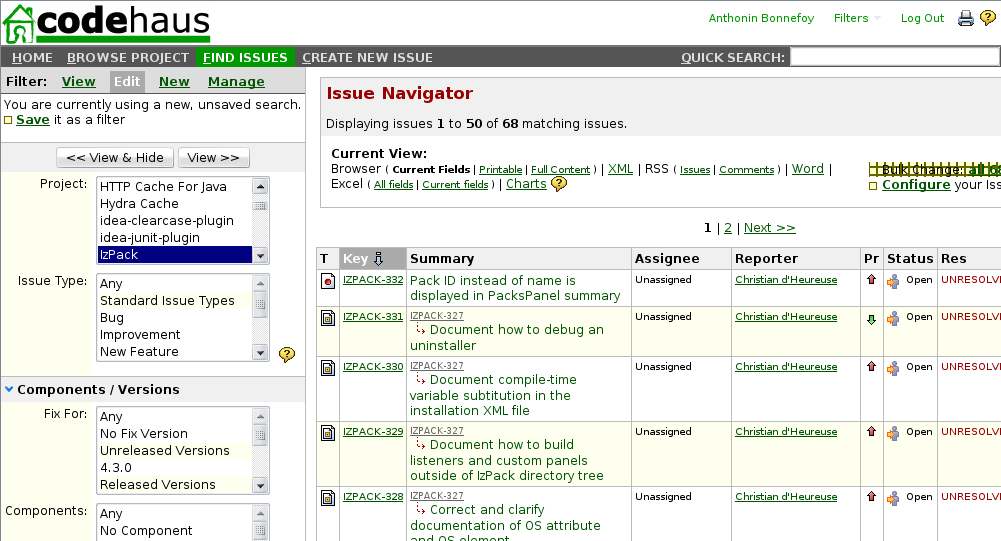
\includegraphics[width=0.8\textwidth]{../image/jira.png}
	\caption{Dashboard Jira}
\end{figure}
\subsection{Suivi de nos apports}
Notre solution étant intégrée, il est possible que des bugs subsistent dans notre implémentation ou qu'une mauvaise interprétation de notre part mène à un comportement inattendu.
Le statut de développeur nous permet de suivre et corriger les problèmes rencontrés par la communauté de IzPack.
\subsubsection{Tests corrigés}
Nous avons par exemple corrigé des tests unitaires sur les numéros de ligne échouant et sur les conditionsTest.
\subsubsection{Rectification sur une interprétation}
Un problème est apparu lors de l'utilisation du Xinclude.
Ce problème a été notifié par un développeur utilisant la version de développement et donc ayant récupéré nos modifications.

Par défaut, Jaxp résout le chemin de manière relative au répertoire d'exécution et c'est ce qui a été réalisée dans notre implementation.
Or le comportement attendu, plus naturel, est de résoudre le chemin d'inclusion relativement au document incluant le xml.

\subsection{Correction de bugs}
Nous avons également corrigé plusieurs bugs.
\subsubsection{Problème lors de l'installation automatique}
Un panel, le TreePacksPanels, ne respectait pas la configuration enregistrée lors de l'installation normale. 
Le problème provenait d'un problème de packaging, la classe devant faire le travail automatique n'était pas présente lors de l'installation.

Un bug caché dans l'installation automatique pouvait la faire quitter silencieusement.
\subsubsection{Web installers}
Izpack possède une fonction de création d'installeurs Web.
Cette fonctionnalité permet de générer des modules d'installations qui pourront être déposés sur un serveur web avec un installeur léger contenant uniquement le noyau dur.
Les modules additionnels seront alors téléchargés s'ils sont sélectionnés.

Cette fonctionnalité présentait des lacunes dans la documentation et n'était pas fonctionnelle.
De plus, un refactoring des classes concernés est en cours de traitement.
\subsubsection{UserInputPanels}
Le panel UserInputPanels doit permettre de décider de l'alignement des éléments.
C'est a dire qu'il est possible de les placer à gauche, à droite ou au centre. Actuellement, tout les éléments sont alignés à gauche.
Le travail est en cours de réalisation mais les modifications entrent en concurrence avec le refactoring de Dennis Reil, un autre contributeur.

\subsection{Améliorations}
Outre les corrections de bugs, la qualité du code a été également amélioré.
Par exemple, le code de l'installeur automatique a été refactoré avec d'autres classes, rendant le code plus lisible et améliorant sa qualité.

De même, certaines méthodes inutilisées (prévues pour des vieilles versions de java) ont pu être supprimées.
%---------------------------------------
\chapter*{Conclusion \markboth{Conclusion}{}}
\addcontentsline{toc}{chapter}{Conclusion}
%------------------------------------------------------------------------------
\begin{frame}<beamer>
\frametitle{Conclusion}
\begin{beamerboxesrounded}[shadow=true]{XML dans IzPack}
\begin{itemize}
	\item NanoXML supprimé
	\item JAXP et ses avantages ajouté
\end{itemize}
\end{beamerboxesrounded}
\vfill
\begin{beamerboxesrounded}[shadow=true]{Contributeurs}
\begin{itemize}
	\item Suivi des apports
	\item Amélioration de IzPack
\end{itemize}
\end{beamerboxesrounded}
\end{frame}
%------------------------------------------------------------------------------
\begin{frame}<beamer>\frametitle{Fin de l'exposé}
\begin{center}
Merci de votre attention.
\end{center}
\end{frame}
%------------------------------------------------------------------------------
\begin{frame}<beamer>\frametitle{Questions}
\begin{center}
Question?
\end{center}
\end{frame}

%---------------------------------------
\chapter*{Glossaire \markboth{Glossaire}{}}
\addcontentsline{toc}{chapter}{Glossaire}
\begin{description}
	\item[packager] Packager est l'action de regrouper en un seul point plusieurs ressources.
	\item[refactoring] C'est une modification du code avec pour but de le rendre plus lisible, maintenable, testable. Il n'ajoute pas de fonctionnalités.
	\item[XML] eXtensible Markup Language. C'est un langage descriptif, qui permet de decrire pratiquement tout. Il est beaucoup utilise dans IzPack.
	\item[fork] Dans GitHub, un fork permet de creer un nouveau depot attache a son compte, dupliquant un autre depot heberge par GitHub.
	\item[W3C] World Wide Web Consortium. C'est le groupe a l'origine de la specification du XML.
\end{description}

%---------------------------------------

\bibliographystyle{alpha}

\begin{btSect}{webographie}
\section*{Webographie}
\section*{Citées}
\btPrintCited
\section*{Non citées}
\btPrintNotCited
\end{btSect}

\begin{btSect}{references}
\section*{Références}
\section*{Citées}
\btPrintCited
\section*{Non citées}
\btPrintNotCited
\end{btSect}
%---------------------------------------
\appendix
\begin{titlepage}
\begin{center}
~\vfill
\hrule
\vfill
\Huge Annexes
\vfill
\hrule
\vfill
\end{center}
\end{titlepage} 
\clearpage
\pagenumbering{Roman}
\chapter*{Annexes}
\setcounter{page}{1}
\addcontentsline{toc}{chapter}{Annexe}
\chapter{Utilisation des éléments nanoXml}

\subsection{Parse par nanoXML}
\begin{verbatim}
	StdXMLParser parser = new StdXMLParser();
	parser.setBuilder(XMLBuilderFactory.createXMLBuilder());
	parser.setReader(new StdXMLReader(in));
	parser.setValidator(new NonValidator());
\end{verbatim}
\subsection{IXMLParser}
3 utilistations
 Utilisé pour parser les fichiers.
 -> com.izforge.izpack.compiler.CompilerConfig
 -> com.izforge.izpack.installer.WebRepositoryAccessor
\subsection{IXMLReader}
5 utilisations
com.izforge.izpack.compiler.CompilerConfig.java
com.izforge.izpack.installer.WebRepositoryAccessor.java
\subsection{NonValidator}
12 utilisations
  com.izforge.izpack
    LocaleDatabase.java
  com.izforge.izpack.compiler
    CompilerConfig.java
  com.izforge.izpack.installer
    AutomatedInstaller.java
    CompileWorker.java
    InstallerFrame.java
    ProcessPanelWorker.java
  com.izforge.izpack.panels
    ShortcutPanel.java
    UserInputPanel.java
  com.izforge.izpack.util
    SpecHelper.java
\subsection{StdXMLParser}
24 utilisations
  com.izforge.izpack
    LocaleDatabase.java 
  com.izforge.izpack.compiler 
    CompilerConfig.java 
  com.izforge.izpack.installer 
    AutomatedInstaller.java 
    CompileWorker.java 
    InstallerFrame.java 
    ProcessPanelWorker.java 
  com.izforge.izpack.panels 
    ShortcutPanel.java 
    UserInputPanel.java 
  com.izforge.izpack.util 
    SpecHelper.java 
\subsection{StdXMLReader}
16 utilisations
  com.izforge.izpack 
    LocaleDatabase.java 
  com.izforge.izpack.compiler 
    CompilerConfig.java 
  com.izforge.izpack.installer 
    AutomatedInstaller.java 
    CompileWorker.java 
    InstallerFrame.java 
    ProcessPanelWorker.java 
    WebRepositoryAccessor.java 
  com.izforge.izpack.panels 
    ShortcutPanel.java 
    UserInputPanel.java 
  com.izforge.izpack.util 
    SpecHelper.java 
\subsection{XMLBuilderFactory}
12 utilisations
  com.izforge.izpack 
    LocaleDatabase.java 
  com.izforge.izpack.compiler 
    CompilerConfig.java 
  com.izforge.izpack.installer 
    AutomatedInstaller.java 
    CompileWorker.java 
    InstallerFrame.java 
    ProcessPanelWorker.java 
  com.izforge.izpack.panels 
    ShortcutPanel.java 
    UserInputPanel.java 
  com.izforge.izpack.util 
    SpecHelper.java 

\subsection{XMLElement}
499 utilisations
\subsection{XMLException}
  com.izforge.izpack.compiler 
    CompilerConfig.java 
\subsection{XMLParserFactory}
3 utilisations
Found usages 
  com.izforge.izpack.compiler 
    CompilerConfig.java 
  com.izforge.izpack.installer 
    WebRepositoryAccessor.java 
\subsection{XMLWriter}
8 utilisations
  com.izforge.izpack.compiler 
    CompilerConfig.java 
    Packager.java 
  com.izforge.izpack.installer 
    InstallerFrame.java 

\end{document}

